\documentclass[12pt, a4paper, oneside]{ctexart}
\usepackage{amsmath, amsthm, amssymb, appendix, bm, graphicx, mathrsfs, geometry, xcolor, subcaption, float, fancyhdr}
\geometry{left=2.54cm, right=2.54cm, top=3.18cm, bottom=3.18cm}
\usepackage[colorlinks, linkcolor=black]{hyperref}

\usepackage{listings}		% 为了避免与页眉的兼容问题可将listings放入table环境中
\lstset{
    basicstyle          =   \sffamily,          % 基本代码风格
    keywordstyle        =   \color{blue},          % 关键字风格
    keywordstyle    =   [2] \color{teal},
    commentstyle        =   \rmfamily\itshape,  % 注释的风格,斜体
    stringstyle         =   \ttfamily,  % 字符串风格
    flexiblecolumns,                % 别问为什么,加上这个
    numbers             =   left,   % 行号的位置在左边
    showspaces          =   false,  % 是否显示空格,显示了有点乱,所以不现实了
    numberstyle         =   \zihao{-5}\ttfamily,    % 行号的样式,小五号,tt等宽字体
    showstringspaces    =   false,
    captionpos          =   t,      % 这段代码的名字所呈现的位置,t指的是top上面
    frame               =   lrtb,   % 显示边框
    basicstyle          =   \zihao{-4}\ttfamily,
    stringstyle         =   \color{magenta},
    commentstyle        =   \color{red}\ttfamily,
    breaklines          =   true,   % 自动换行,建议不要写太长的行
    columns             =   fixed,  % 如果不加这一句,字间距就不固定,很丑,必须加
    basewidth           =   0.5em,
}
\pagestyle{fancy}
\lhead{\textit{\leftmark}}
\chead{} 
\rhead{\textit{\rightmark}}
\lfoot{} 
\cfoot{\thepage}
\rfoot{}
\renewcommand\headrulewidth {0pt} 

\linespread{1.5}
\renewcommand{\abstractname}{\Large\textbf{摘要}}

\begin{document}

\thispagestyle{empty}

\begin{figure}[t]
    \centering
    
\includegraphics[width=13cm]{../pic/xjtu.png}
\end{figure}

\vspace*{\fill}
    \begin{center}
        \centering
        \vspace{-3cm}
        \fangsong\huge{本科生课程报告} \\\kaishu \Huge{\textbf{教育基金会捐助基金管理系统\\的数据流图分析}}
    \end{center}
\vspace*{\fill}

\begin{table}[b]
    \centering
    \large
    \begin{tabular}{ll}
        \textbf{课程:} & 软件系统设计与分析 \\
        \textbf{姓名:} & 杨豪 \\
        \textbf{班级:} & 软件2101 \\
        \textbf{时间:} & 2022年10月 \\
    \end{tabular}
\end{table}

\newpage

\thispagestyle{empty}
\begin{abstract}
    数据流图(DFD, Data Flow Diagram)是结构化分析方法中使用的工具,它以图形的方式从数据的角度描述了一个软件系统,是分析和设计软件系统时一个
    很有用的工具。本文以分析一个切实的软件系统——教育基金会捐助基金管理系统为例,展现了数据流图的基本思想和画法。
    \par\textbf{关键词:}数据流图; 基金管理系统. 
\end{abstract}

\newpage
\pagenumbering{Roman}
\setcounter{page}{1}
\thispagestyle{plain}
\tableofcontents
\newpage
\setcounter{page}{1}
\pagenumbering{arabic}

\section{系统功能分析}

某教育基金会捐助基金管理系统的基本功能如下:
\begin{itemize}
    \item 由捐助者向基金会提出捐助请求,经身份确认后被接受,对捐助人进行登史并授予捐助证书,捐款存入银行;
    \item 由教育单位提出用款申请,在进行相应合法性校验和核对相应的捐款存储后做出支出:
    \item 每月给基金会的理事会一份财政状况报表,列出木月的收入和支出情况利资金余额。
\end{itemize}

故数据流图相关参数如下
\begin{itemize}
    \item 实体:捐助者、教育单位、基金会的理事会;
    \item 信息:捐助者信息、教育单位信息、收支状况信息。
    \item 主要功能:
    \begin{itemize}
        \item 收入处理(输入输出实体均为捐助者):接受请求(捐助请求)、确认身份(和捐助者信息交互)、登记收入(输出信息到收支情况);
        \item 支出处理(输入输出实体均为教育单位):接受请求(用款请求)、合法性检查(和教育单位信息交互)、登记支出(输出信息到收支情况);
        \item 报表输出(无输入,输出实体为基金会的理事会):计时器确定日期、生成财务报表(和收支情况交互)。
    \end{itemize}
\end{itemize}

由此即可构建多级数据流图

\section{多级数据流图}

\subsection{顶层(0层)数据流图}

\begin{figure}[H]
    \centering
    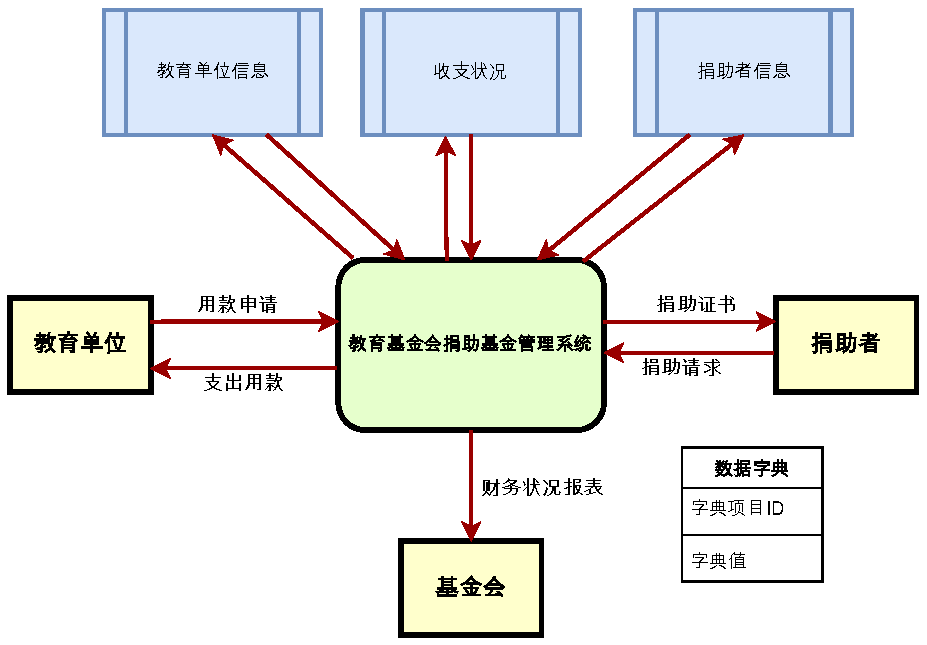
\includegraphics[width = 1\textwidth]{../pic/顶层.pdf}
\end{figure}

\subsection{一层数据流图}

\begin{figure}[H]
    \centering
    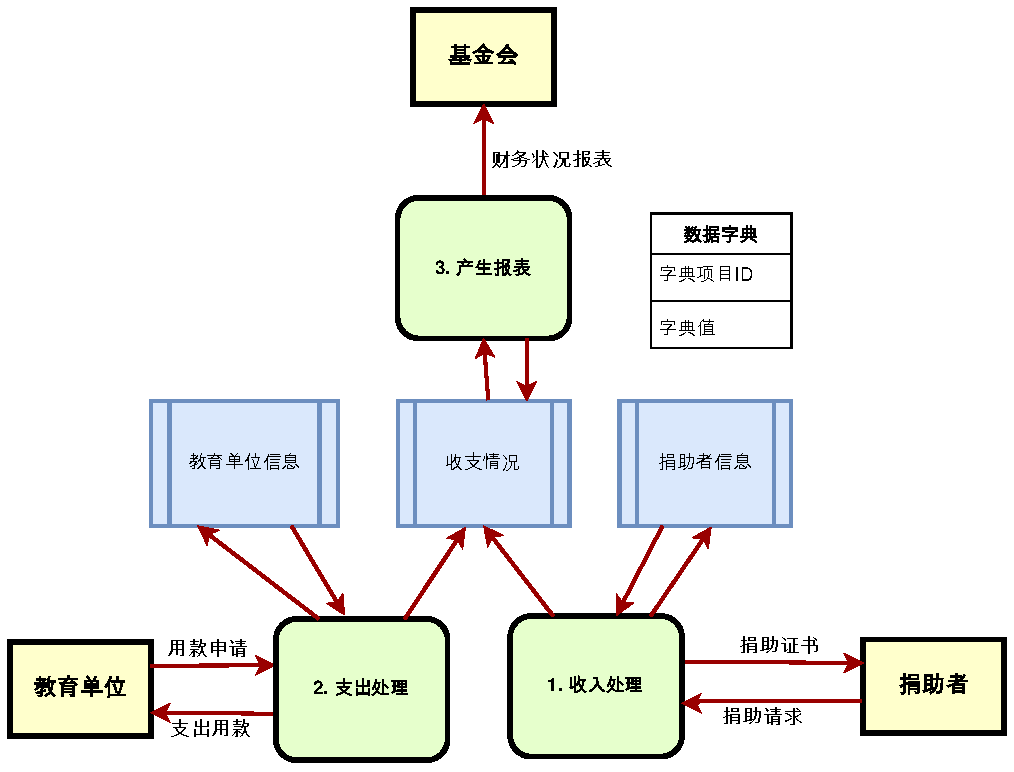
\includegraphics[width = 1\textwidth]{../pic/一级.pdf}
\end{figure}

\subsection{二层数据流图}

\begin{figure}[H]
    \centering
    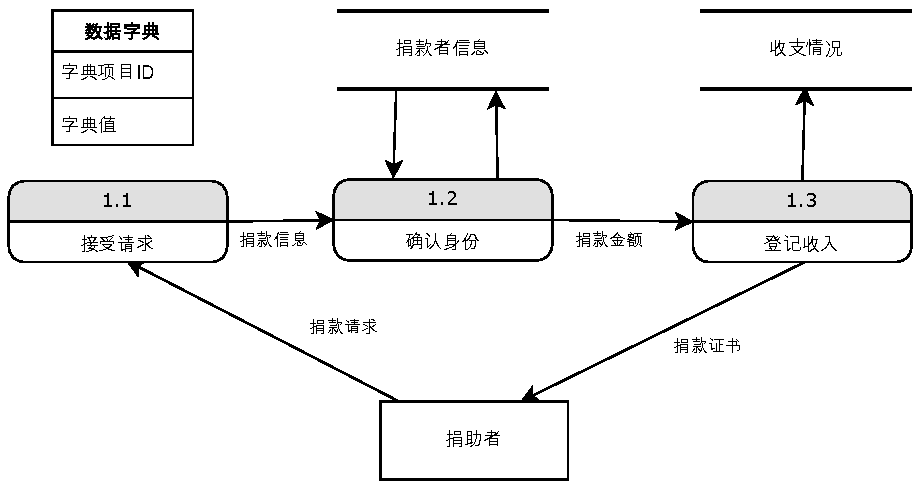
\includegraphics[width = 1\textwidth]{../pic/二级1.pdf}
    \caption{二层数据流图1:收入处理}
\end{figure}

\begin{figure}[H]
    \centering
    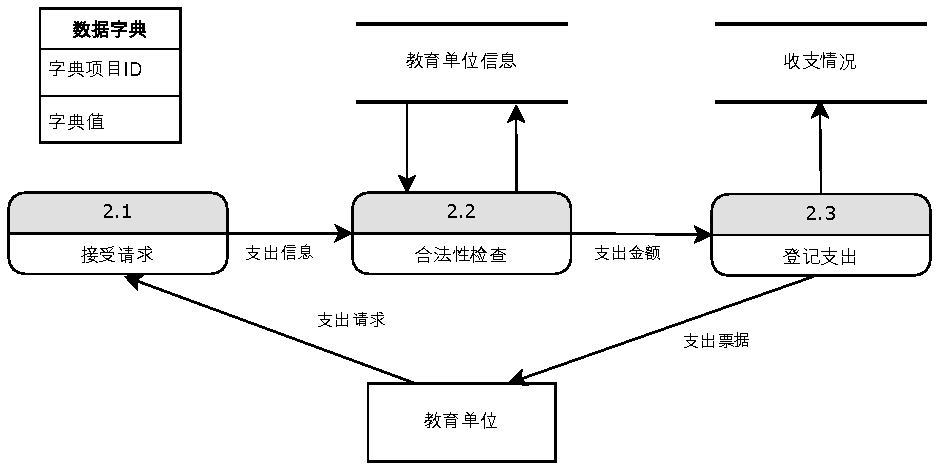
\includegraphics[width = 1\textwidth]{../pic/二级2.pdf}
    \caption{二层数据流图2:支出处理}
\end{figure}

\begin{figure}[H]
    \centering
    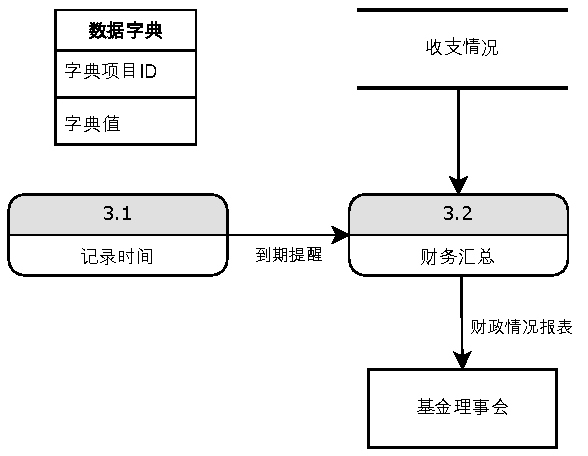
\includegraphics[width = 0.8\textwidth]{../pic/二级3.pdf}
    \caption{二层数据流图3:产生报表}
\end{figure}

\section{总结与体会}

本题目比起作业三简单了许多,我本想使用PowerDesigner制作,但发现PowerDesigner对其支持并不算太优化,所以选择了线上平台~\url{www.iodraw.com}。

由于题目介绍得比较清晰,再加上上课已经练习过更复杂的题目,这道题并没有花费我太多时间,但还是因为没有认真读题导致好几处设计反复修改。
这体现出画图前一定要先认真分析软件系统。

经过对本题和上课时的例题、随堂练习等题目的总结,个人认为数据流图的关键在于三部分:
\begin{itemize}
    \item 外部元素:需要确定系统之外的实体和数据库有哪些。
    \item 划分:除了第一层每一层都需要对上一层划好的分区再次分割,这种对每个区的分割是较难把握的。
    \item 分层:分多少层才好?两层之间的细化不宜太系也不宜太粗,这也很难把握。
\end{itemize}

\end{document}